\documentclass[%
crop,%
tikz,%
convert={outext=.svg,command=\unexpanded{pdf2svg \infile\space../_static/\outfile}},%
multi=false%
]{standalone}%
\usepackage[utf8]{luainputenc}%
\usepackage[no-math]{fontspec}%
\defaultfontfeatures{%
    Numbers={OldStyle,Proportional},%
    Ligatures=TeX,%
    Extension=.ttf,%
}%
\setmainfont[%
UprightFont=*-Regular,%
ItalicFont=*-Italic,%
BoldFont=*-Bold,%
BoldItalicFont=*-BoldItalic,%
]{Raleway}%
\setsansfont[%
UprightFont=*-Regular,%
ItalicFont=*-Italic,%
BoldFont=*-Bold,%
BoldItalicFont=*-BoldItalic,%
]{Raleway}%
\usepackage[frenchmath]{mathastext}%
\usepackage{amsmath}%
\usepackage{amssymb}%
\usepackage{mathrsfs}%
\usepackage{mathtools}%
\usepackage{siunitx}%
\usepackage[siunitx]{circuitikz}%
\usetikzlibrary{calc,backgrounds,arrows.meta,patterns}%

\DeclareMathOperator{\sign}{sign}%

% Ensembles
\let\C\relax
\newcommand{\R}{\ensuremath{\mathbb{R}}} % Réel
\newcommand{\N}{\ensuremath{\mathbb{N}}} % Entiers naturels
% \newcommand{\C}{\ensuremath{\mathbb{C}}} % Complexes
\newcommand{\B}{\ensuremath{\mathscr{B}}} % Bus électriques
\newcommand{\Ch}{\ensuremath{\mathscr{C}}} % Charges
\renewcommand{\L}{\ensuremath{\mathscr{L}}} % Lignes
\renewcommand{\P}{\ensuremath{\mathscr{P}}} % Phases

% Phases
\newcommand{\arm}{\ensuremath{\mathrm{a}}}%
\newcommand{\brm}{\ensuremath{\mathrm{b}}}%
\newcommand{\crm}{\ensuremath{\mathrm{c}}}%
\newcommand{\nrm}{\ensuremath{\mathrm{n}}}%
\newcommand{\trm}{\ensuremath{\mathrm{t}}}%
\newcommand{\grm}{\ensuremath{\mathrm{g}}}%
\newcommand{\abrm}{\ensuremath{\mathrm{ab}}}%
\newcommand{\bcrm}{\ensuremath{\mathrm{bc}}}%
\newcommand{\carm}{\ensuremath{\mathrm{ca}}}%
\newcommand{\anrm}{\ensuremath{\mathrm{an}}}%
\newcommand{\bnrm}{\ensuremath{\mathrm{bn}}}%
\newcommand{\cnrm}{\ensuremath{\mathrm{cn}}}%
\newcommand{\atrm}{\ensuremath{\mathrm{at}}}%
\newcommand{\btrm}{\ensuremath{\mathrm{bt}}}%
\newcommand{\ctrm}{\ensuremath{\mathrm{ct}}}%
\newcommand{\ntrm}{\ensuremath{\mathrm{nt}}}%
\newcommand{\agrm}{\ensuremath{\mathrm{ag}}}%
\newcommand{\bgrm}{\ensuremath{\mathrm{bg}}}%
\newcommand{\cgrm}{\ensuremath{\mathrm{cg}}}%
\newcommand{\ngrm}{\ensuremath{\mathrm{ng}}}%
\newcommand{\abcrm}{\ensuremath{\mathrm{abc}}}%
\newcommand{\abcnrm}{\ensuremath{\mathrm{abcn}}}%

% Indices ou exposants
\newcommand{\cons}{\ensuremath{\mathrm{cons.}}}%
\renewcommand{\prod}{\ensuremath{\mathrm{prod.}}}%
\newcommand{\theo}{\ensuremath{\mathrm{th.}}}%
\newcommand{\const}{\ensuremath{\mathrm{const.}}}%

% Variables
\newcommand{\umax}{\ensuremath{U^{\max}}}%
\newcommand{\umaxnorm}{\ensuremath{U^{\max\,\text{norm.}}}}%
\newcommand{\umin}{\ensuremath{U^{\min}}}%
\newcommand{\uminnorm}{\ensuremath{U^{\min\,\text{norm.}}}}%
\newcommand{\unom}{\ensuremath{U^{\text{nom.}}}}%
\newcommand{\unomnorm}{\ensuremath{U^{\text{nom.}\,\text{norm.}}}}%
\newcommand{\uup}{\ensuremath{U^{\text{up}}}}%
\newcommand{\uupnorm}{\ensuremath{U^{\text{up}\,\text{norm.}}}}%
\newcommand{\uupprime}{\ensuremath{U^{\text{up}\,\prime}}}%
\newcommand{\udown}{\ensuremath{U^{\text{down}}}}%
\newcommand{\udownnorm}{\ensuremath{U^{\text{down}\,\text{norm.}}}}%
\newcommand{\udownprime}{\ensuremath{U^{\text{down}\,\prime}}}%
\newcommand{\smax}{\ensuremath{S^{\max}}}%
\newcommand{\pmax}{\ensuremath{P^{\max}}}%
\newcommand{\sproj}{\ensuremath{\underline{S^{\text{proj.}}}}}%
%

\begin{document}
\ctikzset{american}%
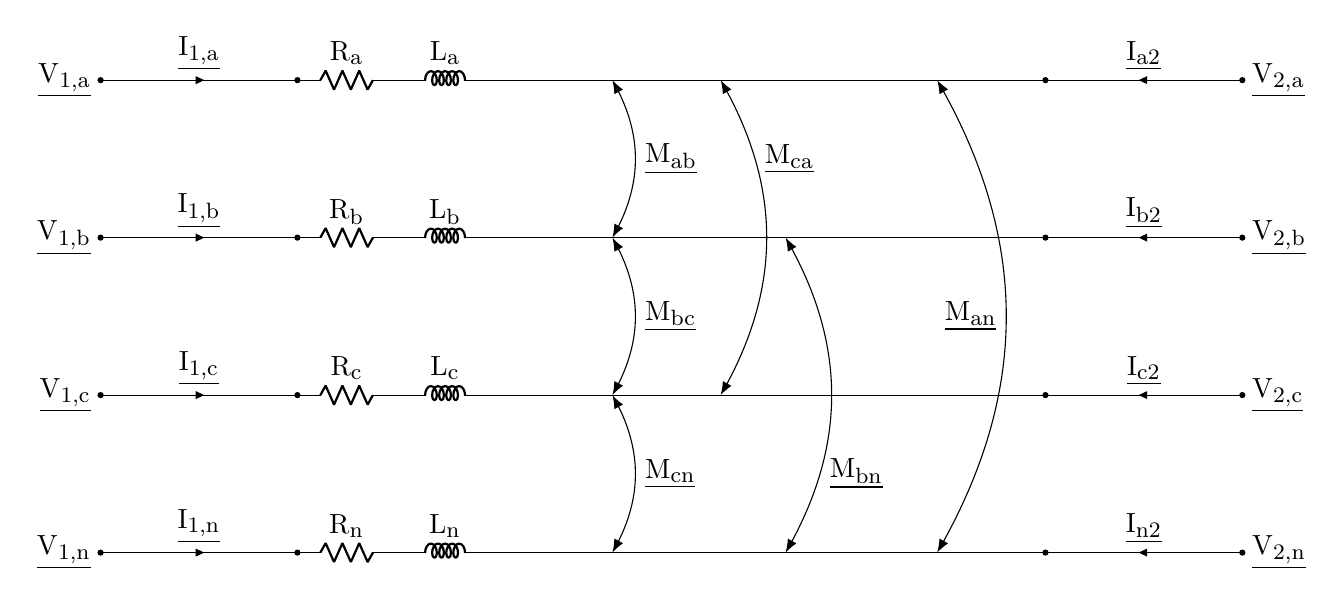
\begin{tikzpicture}[%
    show background rectangle,%
    tight background,%
    background rectangle/.style={fill=white}%
    ]
    % Version multifilaire

    %
    % Définitions
    %
    \pgfmathsetmacro{\xl}{9};%
    \pgfmathsetmacro{\zl}{11.5};%
    \pgfmathsetmacro{\xr}{\zl+2.5};%
    \pgfmathsetmacro{\xri}{\xr+1.5};%
    \pgfmathsetmacro{\zm}{21};%
    \pgfmathsetmacro{\xm}{23.5};%
    \pgfmathsetmacro{\xli}{2.25};%
    \pgfmathsetmacro{\xmi}{\xm-2.25};%
    \pgfmathsetmacro{\yt}{0};%
    \pgfmathsetmacro{\ytt}{-2};%
    \pgfmathsetmacro{\yn}{8};%
    \pgfmathsetmacro{\yc}{10};%
    \pgfmathsetmacro{\yb}{12};%
    \pgfmathsetmacro{\ya}{14};%

    %
    % Styles
    %
    \ctikzset{bipoles/length=0.8cm}%
    \tikzset{fleche/.style={<->,{Latex[]}-{Latex[]}}};%

    %
    % Coordonnées
    %
    \coordinate (orig) at (0,0);

    % Début de ligne
    \coordinate (vlt) at (\xl,\yt);%
    \coordinate (vln) at (\xl,\yn);%
    \coordinate (vlc) at (\xl,\yc);%
    \coordinate (vlb) at (\xl,\yb);%
    \coordinate (vla) at (\xl,\ya);%

    % Fin de ligne
    \coordinate (vmt) at (\xm,\yt);%
    \coordinate (vmn) at (\xm,\yn);%
    \coordinate (vmc) at (\xm,\yc);%
    \coordinate (vmb) at (\xm,\yb);%
    \coordinate (vma) at (\xm,\ya);%

    % Début Z ligne
    \coordinate (zlt) at (\zl,\yt);%
    \coordinate (zln) at (\zl,\yn);%
    \coordinate (zlc) at (\zl,\yc);%
    \coordinate (zlb) at (\zl,\yb);%
    \coordinate (zla) at (\zl,\ya);%

    % Après résistance
    \coordinate (xrt) at (\xr,\yt);%
    \coordinate (xrn) at (\xr,\yn);%
    \coordinate (xrc) at (\xr,\yc);%
    \coordinate (xrb) at (\xr,\yb);%
    \coordinate (xra) at (\xr,\ya);%

    % Après résistance et courant
    \coordinate (xrit) at (\xri,\yt);%
    \coordinate (xrin) at (\xri,\yn);%
    \coordinate (xric) at (\xri,\yc);%
    \coordinate (xrib) at (\xri,\yb);%
    \coordinate (xria) at (\xri,\ya);%

    % Fin Z ligne
    \coordinate (zmt) at (\zm,\yt);%
    \coordinate (zmn) at (\zm,\yn);%
    \coordinate (zmc) at (\zm,\yc);%
    \coordinate (zmb) at (\zm,\yb);%
    \coordinate (zma) at (\zm,\ya);%

    % Première 1/2 admittance
    \coordinate (xlit) at (\xli,\yt);%
    \coordinate (xlin) at (\xli,\yn);%
    \coordinate (xlic) at (\xli,\yc);%
    \coordinate (xlib) at (\xli,\yb);%
    \coordinate (xlia) at (\xli,\ya);%

    % Seconde 1/2 admittance
    \coordinate (xmit) at (\xmi,\yt);%
    \coordinate (xmin) at (\xmi,\yn);%
    \coordinate (xmic) at (\xmi,\yc);%
    \coordinate (xmib) at (\xmi,\yb);%
    \coordinate (xmia) at (\xmi,\ya);%

    % Terre
    \coordinate (g) at (\zl/2+\zm/2,\yt);%
    \coordinate (g2) at (\zl/2+\zm/2,\ytt);%

    %
    % Dessin
    %
    % Tensions amont
    \node[left] at (vla) {$\underline{V_{1,\arm}}$};%
    \node[left] at (vlb) {$\underline{V_{1,\brm}}$};%
    \node[left] at (vlc) {$\underline{V_{1,\crm}}$};%
    \node[left] at (vln) {$\underline{V_{1,\nrm}}$};%

    % Tensions aval
    \node[right] at (vma) {$\underline{V_{2,\arm}}$};%
    \node[right] at (vmb) {$\underline{V_{2,\brm}}$};%
    \node[right] at (vmc) {$\underline{V_{2,\crm}}$};%
    \node[right] at (vmn) {$\underline{V_{2,\nrm}}$};%

    % Câbles principaux
    % Neutre
    \draw (vln) to[short,*-*,i=$\underline{I_{1,\nrm}}$] (zln)
    to[R,l=$R_{\nrm}$] ($(zln)!0.5!(xrn)$) %
    to[L,l=$L_{\nrm}$] (xrn)%
    to[short,-] (xrin) %
    to[short,-*] (zmn)%
    to[short,-*,i<=$\underline{I_{\nrm 2}}$] (vmn);%
    % C
    \draw (vlc) to[short,*-*,i=$\underline{I_{1,\crm}}$] (zlc)%
    to[R,l=$R_{\crm}$] ($(zlc)!0.5!(xrc)$) %
    to[L,l=$L_{\crm}$] (xrc)%
    to[short,-] (xric) %
    to [short,-*] (zmc) %
    to[short,-*,i<=$\underline{I_{\crm 2}}$] (vmc);%
    % B
    \draw (vlb) to[short,*-*,i=$\underline{I_{1,\brm}}$] (zlb)%
    to[R,l=$R_{\brm}$] ($(zlb)!0.5!(xrb)$) %
    to[L,l=$L_{\brm}$] (xrb)%
    to[short,-] (xrib) %
    to[short,-*] (zmb)%
    to[short,-*,i<=$\underline{I_{\brm 2}}$] (vmb);%
    % A
    \draw (vla) to[short,*-*,i=$\underline{I_{1,\arm}}$] (zla)%
    to[R,l=$R_{\arm}$] ($(zla)!0.5!(xra)$)%
    to[L,l=$L_{\arm}$] (xra)%
    to[short,-] (xria) %
    to[short,-*] (zma)%
    to[short,-*,i<=$\underline{I_{\arm 2}}$] (vma);%

    % Mutuelles des lignes
    \pgfmathsetmacro{\xrm}{\xri+0.0*(\zm-\xri)};%
    \draw[fleche] (\xrm,\ya) %
    to[bend left] node[midway,right]{$\underline{M_{\abrm}}$} (\xrm,\yb);%
    \draw[fleche] (\xrm,\yb) %
    to[bend left] node[midway, right]{$\underline{M_{\bcrm}}$} (\xrm,\yc);%
    \draw[fleche] (\xrm,\yc) %
    to[bend left] node[midway,right]{$\underline{M_{\cnrm}}$} (\xrm,\yn);%
    \pgfmathsetmacro{\xrm}{\xri+0.25*(\zm-\xri)};%
    \draw[fleche] (\xrm,\ya) %
    to[bend left] node[near start,right]{$\underline{M_{\carm}}$} (\xrm,\yc);%
    \pgfmathsetmacro{\xrm}{\xri+0.40*(\zm-\xri)};%
    \draw[fleche] (\xrm,\yb) %
    to[bend left] node[near end,right]{$\underline{M_{\bnrm}}$} (\xrm,\yn);%
    \pgfmathsetmacro{\xrm}{\xri+0.75*(\zm-\xri)};%
    \draw[fleche] (\xrm,\ya) %
    to[bend left] node[midway,left]{$\underline{M_{\anrm}}$} (\xrm,\yn);%

\end{tikzpicture}
\end{document}
% Local Variables:
% mode: latex
% TeX-engine: luatex
% TeX-source-correlate-method-active: synctex
% ispell-local-dictionary: "british"
% coding: utf-8
% LaTeX-indent-level: 4
% fill-column: 100
% End:
